\documentclass[t, 9pt]{beamer}
\mode<presentation>
{
  \usetheme{Warsaw}
  %\usefonttheme{serif}
}
\setbeamertemplate{caption}[numbered]
%\mode<presentation>
%{
%\usetheme{Warsaw}
%}
%\usefonttheme{structuresmallcapsserif}

%----------------------------------------
%            PACKAGES
%----------------------------------------

%--FIGURES
%\usepackage{graphicx}
\usepackage{subfigure}

%--FONT
%\usepackage{textcomp} 
\usepackage{amsmath}
\numberwithin{equation}{section}
\usepackage{amssymb}
\usepackage[bold]{hhtensor}
\usepackage{array}
%-----TIKZ
\usepackage{circuitikz}
\usepackage{ifthen}
\usepackage{tikz}
\usepackage{pgf}
\usepackage{pgffor}
\usepgfmodule{shapes}
\usepgfmodule{plot}
\usetikzlibrary{decorations}
\usetikzlibrary{arrows}
\usetikzlibrary{snakes}
\usetikzlibrary{arrows,positioning} 
\tikzset{
    %Define standard arrow tip
    >=stealth',
    %Define style for boxes
    punkt/.style={
           rectangle,
           rounded corners,
           draw=black, very thick,
           text width=6.5em,
           minimum height=2em,
           text centered},
    % Define arrow style
    pil/.style={
           ->,
           thick,
           shorten <=2pt,
           shorten >=2pt,}
}

\usepackage{xcolor}
\def\setcolormodel{cmyk}

%--HYPERLINKS
%\hypersetup{colorlinks=true,       % false: boxed links; true: colored links
%	linkcolor=OliveGreen,          % color of internal links
%	citecolor=BrickRed,        % color of links to bibliography
%	urlcolor=Blue,
%	bookmarksnumbered=true,
%	pdffitwindow=true, 
%	bookmarks=true}         % show
%\usepackage{url}

%--GRAPHICS PATH
\graphicspath{{~/Dropbox/github/TOM/figures/}}



%--Title slide configuration
%% !TEX root = F429_1s1014.tex

\title[]{Alternate Currents \& Optics - F 429}

\author[Gustavo Wiederhecker]{
Gustavo Wiederhecker\\
\vspace{10pt}
some extra text 3
}
\date{March 2014}


%--BEGIN DOCUMENT HERE!
\begin{document}  
% Shortcut fot tables and figures.
\def\figurename{Fig.}
\def\tablename{Tab.}  
\ctikzset{bipoles/length=.7cm}

%---------------------------------------------------------------------
%            SHORTCUTS USED IN THE TEXT
%---------------------------------------------------------------------
% CUSTOM SHORTCUTS
\newcommand{\neff}{n_\text{eff}}
\newcommand{\ml}{Matlab\textsuperscript{\textregistered} }
\newcommand{\cm}{Comsol\textsuperscript{\textregistered} }
\newcommand{\sinn}{Si$_3$N$_4$\text{ }}
\newcommand{\sio}{SiO$_2$\text{ }}
%
%\newcommand*{\eps0}{ \epsilon_0 }
%\newcommand{\mu0}{\mu$_0$}

%------------------------------------------
%vector calculus
\newcommand{\divg}[1]{\nabla \cdot \vec{#1}}
\newcommand{\rot}[1]{\nabla \times \vec{#1}}

%------------------------------------------
%time derivatives
\newcommand{\dpt}[1]{\frac{\partial \vec{#1}}{\partial t}}
\newcommand{\dt}[1]{\frac{d \vec{#1}}{d t}}

%------------------------------------------
%			TWO PORT NETWORK
%------------------------------------------
\newcommand{\tpn}[2]{
	\begin{circuitikz}[scale=1]
		\node (Xi) at (0.7,0.7) {$V_1$};
		\node (Xf) at (3.7,0.7) {$V_2$};
		\draw [semithick,->] (Xi) -- (0.1,0.1);
		\draw [semithick,->] (Xf) -- (3.1,0.1);
		\draw
			to [generic, o-o, l_=$#1$] ++(2,0)
			(2,0) to [short,o-o] ++(1,0)
			(2,0) to [generic, o-o, l=$#2$] ++(0,-2)
			node[ground] {}
			;
	\end{circuitikz}
}

\newcommand{\tpn}[2]{
	\begin{circuitikz}[scale=1]
		\node (Xi) at (0.7,0.7) {$V_1$};
		\node (Xf) at (3.7,0.7) {$V_2$};
		\draw [semithick,->] (Xi) -- (0.1,0.1);
		\draw [semithick,->] (Xf) -- (3.1,0.1);
		\draw
			to [generic, o-o, l_=$#1$] ++(2,0)
			(2,0) to [short,o-o] ++(1,0)
			(2,0) to [generic, o-o, l=$#2$] ++(0,-2)
			node[ground] {}
			;
	\end{circuitikz}
}	
%------------------------------------------
%			PHASOR DIAGRAM
%------------------------------------------
\newcommand{\Gitter}[4]{
    \draw[very thin,color=gray] (#1,#3) grid (#2,#4);
}
\newcommand{\Koordinatenkreuz}[6]{
    \draw[->, >=latex, color=green!50!black] (#1,0) -- (#2,0) node[right] {#5};
    \draw[->, >=latex, color=green!50!black] (0,#3) -- (0,#4) node[left] {#6};
}
\newcommand{\KoordinatenkreuzOhneLabelsVerschobenKeinPfeil}[5]{
    \draw[-] (#1,0) -- (#2,0);
    \draw[-] (#5,#3) -- (#5,#4);

}
\newcommand{\ZeigerdiagrammText}[4]{
\begin{tikzpicture}[scale=.72, samples=100, >=latex]

    \def\Alpha{#1}
    \def\Phase{#2}
    \def\AmplitudeSpannung{#3}
    \def\AmplitudeStrom{#4}
    \def\SpannungsWert{{\AmplitudeSpannung*sin(\Alpha)}}
    \def\StromWert{{\AmplitudeStrom*sin(\Alpha+\Phase)}}
    %%%%%%%%%%%%%%%%%%%%%%%%%%%%%%%%%%%%%%%%%%%%%%%%%%%%%%%%%%
    \def\FarbeSpannung{blue!90!white}
    \def\FarbeStrom{red!90!white}
    \def\FarbeWinkelZeichnung{green}
    %%%%%%%%%%%%%%%%%%%%%%%%%%%%%%%%%%%%%%%%%%%%%%%%%%%%%%%%%%
    \def\Beta{\Alpha+\Phase}
    \def\AlphaRad{\Alpha*3.141592654/180}
    \def\PhaseRad{\Phase*3.141592654/180}
    %%%%%%%%%%%%%%%%%%%%%%%%%%%%%%%%%%%%%%%%%%%%%%%%%%%%%%%%%%
    \Gitter{-.1}{7.1}{-3.1}{3.1}
    \Koordinatenkreuz{-.2}{7.3}{-3.2}{3.3}{$\omega t$}{}
    \draw (1.570795,0) node[below]{$\frac{\pi}{2}$};
    \draw (3.14159,0) node[below]{${\pi}$};
    \draw (4.71238898,0) node[below]{$\frac{3\pi}{2}$};
    \draw (6.283185307,0) node[below]{${2\pi}$};
    \draw (-4,0) circle (3cm);
    \KoordinatenkreuzOhneLabelsVerschobenKeinPfeil{-7.2}{-.8}{-3.6}{3.6}{-4}
    %%%%%%%%%%%%%%%%%%%%%%%%%%%%%%%%%%%%%%%%%%%%%%%%%%%%%%%%%%

    % voltage
    \draw[color=\FarbeSpannung, very thick] plot[id=voltage, domain=0:7] function{\AmplitudeSpannung*sin(x)} node[right] {$U(t)$};
    % voltage circle
    \draw[color=\FarbeSpannung, loosely dashed] (-4,0) circle (\AmplitudeSpannung cm);
    % angle
    \draw[color=\FarbeWinkelZeichnung!50!black, thick] (\AlphaRad, \SpannungsWert)--(\AlphaRad,\StromWert) node[below=18pt] {$\alpha$};
    % angle in the circle
    \filldraw[fill=\FarbeWinkelZeichnung!20,draw=\FarbeWinkelZeichnung!50!black] (-4,0) -- (-3,0) arc (0:\Alpha:1) -- cycle node[right] {$\alpha$};
    % voltage pointer
    \draw[<-,color=\FarbeSpannung, very thick] (\Alpha:\AmplitudeSpannung)++(-4,0) --(-4,0);
    \draw[color=\FarbeSpannung,  dashed] (\Alpha:\AmplitudeSpannung)++(-4,0) -- (\AlphaRad,\SpannungsWert);
    % current
    \draw[color=\FarbeStrom, very thick] plot[id=current, domain=0:7] function{\AmplitudeStrom*sin(x+\PhaseRad)} node[right] {$I(t)$};		
    % current circle
    \draw[color=\FarbeStrom, loosely dashed]    (-4,0) circle (\AmplitudeStrom cm);
    % current pointer
    \draw[<-,color=\FarbeStrom, very thick] (\Beta:\AmplitudeStrom)++(-4,0) --(-4,0);
    \draw[color=\FarbeStrom,  dashed](\Beta:\AmplitudeStrom)++(-4,0) -- (\AlphaRad,\StromWert);
    % phase difference
    \ifthenelse{\Phase<0}{
        \draw[snake=brace] (pi/2 ,3.3)--(pi/2-\PhaseRad ,3.3) node[above=7pt, left=10pt] {$\phi$};
    }
    {
        \draw[snake=brace] (pi/2-\PhaseRad ,3.3)--(pi/2 ,3.3) node[above=7pt, left=10pt] {$\phi$};
    }
    % angular velocity \omega
    \draw[->, xshift=-4cm]  (120:2.4cm) arc (120:170:2) node[below] {$\omega$};
\end{tikzpicture}
}




%----------------------------------------
%-- SLIDES BEGIN HERE!!
%----------------------------------------

% Title slide
\begin{frame}
  \titlepage
\end{frame}

\AtBeginSection[]
{
\begin{frame}<beamer>{Table of Contents}
\tableofcontents[currentsection,currentsubsection, 
    hideothersubsections, 
    sectionstyle=show/shaded,
]
\end{frame}
}

% Maxwell Equations
%\subsection{Generic two-port circuits}
\begin{frame}{Generic two-port circuits}
During the next experiments we will explore a few configurations of two-port circuits. The typical setup will be similar to Fig. \ref{fig:Generic_two_port} below.
\begin{figure}[hbt]
	\begin{circuitikz}
		\draw
			(0,0) node[ground] {}
			to [sinusoidal voltage source, o-o, l=$\epsilon(t)$] ++(0,2)
			to [generic, o-o, l=$Z_g$] ++(2,0)
			to [generic, o-o, l=$Z_1$] ++(2,0)
			(4,2) to [short,o-o,l_=a] ++(1,0)
			(4,2) to [generic, o-o, l=$Z_2$] ++(0,-2)
			node[ground] {}
			;
		%Description of subparts
		\draw [decorate,decoration={brace,amplitude=8pt},
					xshift=0pt, yshift=0pt]
					(2,-1) -- (-0.5,-1)
					node[black,midway,yshift=-20pt]
						{AC generator};
		\draw [decorate,decoration={brace,amplitude=8pt},
					xshift=0pt, yshift=0pt]
					(5,-1) -- (2.1,-1)
					node[black,right,yshift=-20pt]
						{Two-port circuit};	
	\end{circuitikz}
  \caption{\tiny{Generic two-port circuit setup. $Z_g$ represents the internal impedance of the AC generators, $Z_1,Z_2$ are any generic linear circuit components. The arrows $V_1$ and $V_2$ indicate where we connect  oscilloscope channels to the circuit. }}
  \label{fig:Generic_two_port}
\end{figure}

\end{frame}

\begin{frame}{Resistive voltage divider}
The simplest example of a two-port circuit is the voltage divider 			you learned in F328/F329 \cite{Walker:2008aa}. You obtain it by 			simple replacing $Z_{1,2}$ from Fig. \ref{fig:Generic_two_port} with two resistors.
	\begin{columns}
		\begin{column}{0.5\textwidth}
			\tpn{R_1}{R_2}
				\end{column}
		\begin{column}{0.5\textwidth}
		From KCL (Kirchhoff Circuit's Law):
			\begin{eqnarray}
			\Rightarrow v_1(t)=R_1 i(t)+ R_2 i(t)\\
			\Rightarrow i(t)=\frac{v_1(t)}{R_1+R_2}
			\label{eq:voltagediv_i}
  			\end{eqnarray}
		The voltage drop measured in channel 2 is given by
		\begin{equation}
  			v_2(t)=R_2 i(t)=\frac{R_2}{R_1+R_2}v_1(t)
  			\label{eq:voltagediv_v2}
		\end{equation}
		
		\end{column}
	\end{columns}
\end{frame}

\begin{frame}{Resistive voltage divider}
Based on Eq. \ref{eq:voltagediv_v2}, it is obvious now why such a circuit is called the voltage divider; the voltage measured on the \textbf{output port} of the circuit ($v_2$) is a fraction of the \textbf{input port} voltage ($v_1$).
	\begin{columns}
		\begin{column}{0.4\textwidth}
			\tpn{R_1}{R_2}
		\end{column}
		\begin{column}{0.6\textwidth}
		Using Eqs. \ref{eq:voltagediv_i} and \ref{eq:voltagediv_v2} one can now define the \textbf{frequency response} of the resistive voltage divider. For a given sinusoidal input, $v_1(t)=V_1\sin(\omega t)$, the output voltage will be given by 
\begin{equation}
  v_2(t)=\frac{R_2}{R_1+R_2}V_1\sin(\omega t)
  \label{eq:voltagediv_v2_freq}
\end{equation}
From Eq. \ref{eq:voltagediv_v2_freq} it is clear that the output voltage is \textbf{in-phase} with the input voltage but with a different amplitude.

		\end{column}
	\end{columns}
\end{frame}

\begin{frame}{Resistive voltage divider}
One can then define an output voltage $v_2(t)=V_2\sin(\omega t)$, where the amplitude $V_2=\frac{R_2}{R_1+R_2}V_1$. We now define a important quantity:
\begin{definition}
The response function of the two-port circuit network $H(\omega)$ is input-output relation $H(\omega)\equiv\frac{V_2(\omega)}{V_1(\omega)}$.
\end{definition}
Note however that although we included an explicit frequency dependence on the $H(\omega)$, in the trivial case of the resistive voltage divider $H=R_2/(R_1+R_2)$ does not depend on frequency. That simply reflects the fact that the voltage drop in a resistor is proportional to the current flowing through it.\\ In the laboratory it means that regardless of the AC generator frequency, the ratio of the voltage amplitudes measured in channels 1,2 will always be given by  $R_2/(R_1+R_2)$.
%		\begin{columns}
%			\begin{column}{0.5\textwidth}
%				\tpn{R_1}{R_2}
%			\end{column}
%			\begin{column}{0.5\textwidth}
%			
%			\end{column}
%		\end{columns}
\end{frame}

\begin{frame}{Resistive voltage divider: Numerical example}

\end{frame}

\subsection{RC voltage divider - Filters}

\begin{frame}{RC voltage divider}
We can try to apply the same principles used in the resistive voltage divider to a slightly more complex one, involving both a resistor and a capacitor. You shold also have learned about this circuit in F328/F329 \cite{Walker:2008aa}. You obtain it by 			simple replacing $Z_{1,2}$ from Fig. \ref{fig:Generic_two_port} with a capacitor and a resistor.
	\begin{columns}
		\begin{column}{0.5\textwidth}
			\tpn{R}{C}
			\tpn{C}{R}
				\end{column}
		\begin{column}{0.5\textwidth}
		From KCL (Kirchhoff Circuit's Law):
			\begin{equation}
			\Rightarrow v_1(t)=R i(t)+  q(t)/C
			\label{eq:rc_1}
  			\end{equation}
  			In contrast with the resistive divider (Eq. \ref{eq:voltagediv_i}), Eq. \ref{eq:rc_1} is an ordinary differential equation (ODE). Note that either circuit shown in the left follows the same equation. The difference is the voltage drop measured in channel 2 which will be given by
		\begin{eqnarray}
		     v_2(t)=q(t)/C\\
		     v_2(t)=R i(t)
  			\label{eq:rc_v2}
		\end{eqnarray}
		
		\end{column}
	\end{columns}
\end{frame}

\begin{frame}{RC voltage divider}
In order for to Eqs. \ref{eq:rc_v2} to be useful, one must solve the ODE \ref{eq:rc_1}. It is a inhomogeneous ODE where the dependent variable is the charge $q(t)$. We can decompose its solution in two parts, $q(t)=q_h(t)+q_p(t)$, where $q_h(t)=q_0 \exp(-t/\tau)$ is the solution of the homogenous equation ($v_1=0$) and $q_p(t)=$ust have In the particular case of sinusoidal input, $v_1(t)=V_1\sin(\omega t)$, 
\end{frame}

\begin{figure}


%(0,0) node[ground] {} (0,0)
%to [sinusoidal voltage source, o-o, l=$\epsilon(t)$] ++(0,2)
%to [R, o-o, l=$R_g$] ++(2,0)
%to [generic, o-o, l=$Z_1$] ++(2,0)
%to [generic, o-o, l=$Z_2$] --(0,2)
%;

\section{Two-port circuits}
\subsection{Generic two-port circuits}
\begin{frame}{Generic two-port circuits}
\label{fr:twoport}
During the next experiments we will explore a few configurations of two-port circuits. The typical setup will be similar to Fig. \ref{fig:Generic_two_port} below. 
\hyperlink{fr:appendix1}{\beamerbutton{here}}.
\begin{figure}[hbt]
\begin{circuitikz}[scale=0.5]
		\draw
			(0,0) node[ground] {}
			to [sinusoidal voltage source, o-o, l=$\epsilon(t)$] ++(0,2)
			to [generic, o-o, l=$Z_g$] ++(2,0)
			to [generic, o-o, l=$Z_1$] ++(2,0)
			(4,2) to [short,o-o] ++(1,0)
			(4,2) to [generic, o-o, l=$Z_2$] ++(0,-2)
			node[ground] {}
			;
		%Description of subparts
		\draw [decorate,decoration={brace,amplitude=8pt},
					xshift=0pt, yshift=0pt]
					(2,-1) -- (-0.5,-1)
					node[black,midway,yshift=-20pt]
						{AC generator};
		\draw [decorate,decoration={brace,amplitude=8pt},
					xshift=0pt, yshift=0pt]
					(5,-1) -- (2.1,-1)
					node[black,right,yshift=-20pt]
						{Two-port circuit};	
	\end{circuitikz}
  \caption{\tiny{Generic two-port circuit setup. $Z_g$ represents the internal impedance of the AC generators, $Z_1,Z_2$ are any generic linear circuit components. The arrows $V_1$ and $V_2$ indicate where we connect  oscilloscope channels to the circuit. }}
  \label{fig:Generic_two_port}
\end{figure}

\end{frame}

\begin{frame}{Resistive voltage divider}
The simplest example of a two-port circuit is the voltage divider you learned in F328/F329 \cite{Walker:2008aa}. You obtain it by simple replacing $Z_{1,2}$ from Fig. \ref{fig:Generic_two_port} with two resistors
	\begin{columns}
	\vspace{10pt}
		\begin{column}{0.5\textwidth}
		\tpn{R_1}{R_2}
		From KCL (Kirchhoff Circuit's Law)
		\begin{eqnarray}
		\Rightarrow v_1(t)=R_1 i(t)+ R_2 i(t)\\
		\Rightarrow i(t)=\frac{v_1(t)}{R_1+R_2}\label{eq:voltagediv_i}
		\end{eqnarray}
		\end{column}
		\pause
		\begin{column}{0.5\textwidth}
		The voltage drop measured in channel 2 is given by
		\begin{equation}
		v_2(t)=R_2 i(t)=\frac{R_2}{R_1+R_2}v_1(t)
		\label{eq:voltagediv_v2}
		\end{equation}
		Based on Eq. \ref{eq:voltagediv_v2}, it is obvious now why such a circuit is called the voltage divider; the voltage measured on the \textbf{output port} of the circuit ($v_2$) is a fraction of the \textbf{input port} voltage ($v_1$).

		\end{column}
	\end{columns}
\end{frame}


%\begin{columns}
%	\begin{column}{0.5\textwidth}
%	
%		\tpn{R_1}{R_2}
%	\end{column}
%	\begin{column}{0.5\textwidth}
%	%\pause

%	\end{column}
%	\end{columns}
%\end{frame}


\begin{frame}{Resistive voltage divider}
\begin{columns}
	\begin{column}{0.4\textwidth}
		\tpn{R_1}{R_2}
		Using Eqs. \ref{eq:voltagediv_i} and \ref{eq:voltagediv_v2} one can now define the \textbf{frequency response} of the 	resistive voltage divider.
	\end{column}
	\begin{column}{0.6\textwidth}
		 For a given sinusoidal input, $v_1(t)=V_1\sin(\omega t)$, the output voltage will be given by 
\begin{equation}
	v_2(t)=\frac{R_2}{R_1+R_2}V_1\sin(\omega t)
 	\label{eq:voltagediv_v2_freq}
\end{equation}
From Eq. \ref{eq:voltagediv_v2_freq} it is clear that the output voltage is \textbf{in-phase} with the input voltage but with a different amplitude. One can then define an output voltage $v_2(t)=V_2\sin(\omega t)$, where the amplitude $V_2=\frac{R_2}{R_1+R_2}V_1$. We now define a important quantity:
\begin{definition}
The response function of the two-port circuit network $H(\omega)$ is the input-output relation between the voltage amplitudes, $H(\omega)\equiv\frac{V_2(\omega)}{V_1(\omega)}$.
\end{definition}
	\end{column}
\end{columns}

\end{frame}

\begin{frame}{Resistive voltage divider}


Note however that although we included an explicit frequency dependence on the $H(\omega)$, in the trivial case of the resistive voltage divider $H=R_2/(R_1+R_2)$ does not depend on frequency. That simply reflects the fact that the voltage drop in a resistor is proportional to the current flowing through it.\\ In the laboratory it means that regardless of the AC generator frequency, the ratio of the voltage amplitudes measured in channels 1,2 will always be given by  $R_2/(R_1+R_2)$.
\begin{example}
\begin{columns}

\begin{column}{0.3\textwidth}
\begin{center}
\begin{circuitikz}[scale=0.5]
	\draw
		(0,0) node[ground] {}
		to [sinusoidal voltage source, o-o, l=$\epsilon(t)$] ++(0,2)
		to [resistor, o-o, l=$R_g$] ++(2,0)
		(2,2) to [short,o-o] ++(1,0)
		(2,2) to [resistor, o-o, l=$R$] ++(0,-2)
		node[ground] {}
		;
\end{circuitikz}
\end{center}
\end{column}

\begin{column}{0.65\textwidth}
Suppose we want to measure to internal impedance of a given AC source. 
\end{column}

\end{columns}

\end{example}

%		\begin{columns}
%			\begin{column}{0.5\textwidth}
%				\tpn{R_1}{R_2}
%			\end{column}
%			\begin{column}{0.5\textwidth}
%			
%			\end{column}
%		\end{columns}
\end{frame}

\begin{frame}{Resistive voltage divider: Numerical example}

\end{frame}

\subsection{RC voltage divider - Filters}

\begin{frame}{RC voltage divider}
We can try to apply the same principles used in the resistive voltage divider to a slightly more complex one, involving both a resistor and a capacitor. You shold also have learned about this circuit in F328/F329 \cite{Walker:2008aa}. You obtain it by 			simple replacing $Z_{1,2}$ from Fig. \ref{fig:Generic_two_port} with a capacitor and a resistor.
	\begin{columns}
		\begin{column}{0.5\textwidth}
			\tpn{R}{C}
			\tpn{C}{R}
				\end{column}
		\begin{column}{0.5\textwidth}
		From KCL (Kirchhoff Circuit's Law):
			\begin{equation}
			\Rightarrow v_1(t)=R i(t)+  q(t)/C
			\label{eq:rc_1}
  			\end{equation}
  			In contrast with the resistive divider (Eq. \ref{eq:voltagediv_i}), Eq. \ref{eq:rc_1} is an ordinary differential equation (ODE). Note that either circuit shown in the left follows the same equation. The difference is the voltage drop measured in channel 2 which will be given by
		\begin{eqnarray}
		     v_2(t)=q(t)/C\label{eq:rc_v2c}\\
		     v_2(t)=R i(t)
  			\label{eq:rc_v2r}
		\end{eqnarray}
		
		\end{column}
	\end{columns}
\end{frame}

\begin{frame}{RC voltage divider}
In order to Eqs. \ref{eq:rc_v2c},\ref{eq:rc_v2r} be useful, one must solve the ODE \ref{eq:rc_1}. It is a inhomogeneous ODE where the dependent variable is the charge $q(t)$. We can decompose its solution in two parts, $q(t)=q_h(t)+q_p(t)$, where $q_h(t)=q_0 \exp(-t/\tau)$ is the solution of the homogenous equation ($v_1=0$) and $q_p(t)$ is a particular solution which depends on the explicit form of the driving term $v_1(t)$. After the initial transients $q_h(t)$ decays and \textbf{the only important contribution is due to} $q_p(t)$. This is also called the \textbf{steady-state}.

For $v_1(t)=V_1\cos(\omega t)$ the solution is given by, 
\begin{equation}
i_p(t)=\frac{\omega C V_1 }{1+\omega^2 R^2 C^2}(\omega R C\cos(\omega t)-\sin(\omega t))=\frac{\omega C V_1 }{\sqrt{1+\omega^2 R^2 C^2}}\cos(\omega t +\phi)
\label{eq:rc_solpart}
\end{equation}
where $\phi=\tan^{-1}(\frac{1}{\omega R C})$. With Eq. \ref{eq:rc_solpart} in hand we may be tempted to proceed similarly to the resistive divider in order to derive the transfer function $H(\omega)$. Using Eqs. \ref{eq:rc_v2c},\ref{eq:rc_v2r} we obtain,
\begin{eqnarray}
v_2^{(C)}(t)=\frac{-1}{\sqrt{1+\omega^2 R^2 C^2}} V_1 \sin(\omega t +\phi) \label{eq:rc_v2final_c}\\
v_2^{(R)}(t)=\frac{\omega R C }{\sqrt{1+\omega^2 R^2 C^2}} V_1 \cos(\omega t +\phi) \label{eq:rc_v2final_r}
\end{eqnarray}

\end{frame}

\begin{frame}{RC voltage divider}
From Eq.\ref{eq:rc_v2final_c} we learn a lot about how the circuit respond to a sinusoidal excitation. In Figs. \ref{fig:bodepa_lin},\ref{fig:bodepa_log} below we plot them ($v_2^{(R)}$) in the so-called \textbf{Bode Diagrams}. Note the extra information avaliable in the $\log$ version!
	\begin{columns}
		\begin{column}{0.5\textwidth}
			\begin{figure}
  			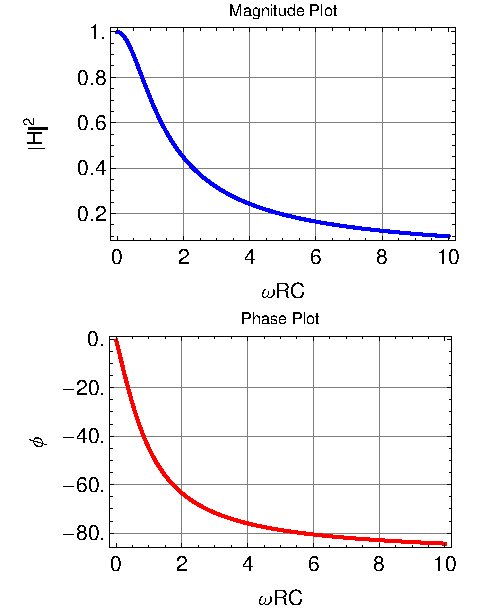
\includegraphics[width=0.7\textwidth]{bodepb_lin.pdf}
  			\caption{Linear Bode plots, $|H|^2=\frac{1}{1+\omega^2 R^2 C^2},\phi=tan^{-1}(1/\omega RC)$}
  			\label{fig:bodepb_lin}
			\end{figure}
		\end{column}
		\begin{column}{0.5\textwidth}
			\begin{figure}
  			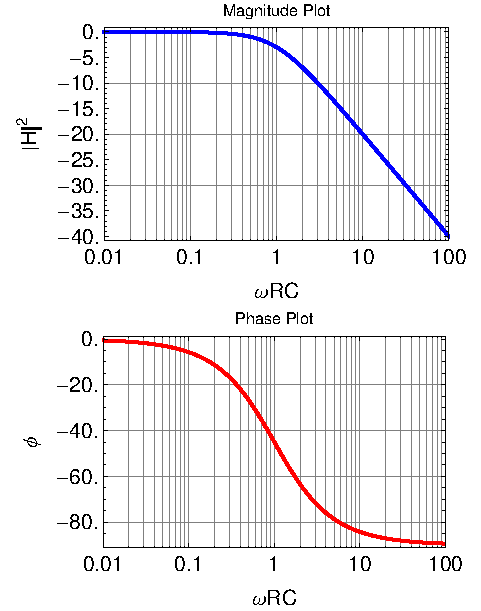
\includegraphics[width=0.7\textwidth]{bodepb_log.pdf}
  			\caption{Log Bode plots, $|H|^2=\frac{1}{1+\omega^2 R^2 C^2},\phi=tan^{-1}(1/\omega RC)$}
  			\label{fig:bodepb_log}
			\end{figure}
		\end{column}
	\end{columns}
\end{frame}

\begin{frame}{RC voltage divider}
From Eq.\ref{eq:rc_v2final_r} we learn a lot about how the circuit respond to a sinusoidal excitation. In Figs. \ref{fig:bodepa_lin},\ref{fig:bodepa_log} below we plot them ($v_2^{(C)}$) in the so-called \textbf{Bode Diagrams}. Note the extra information avaliable in the $\log$ version!
	\begin{columns}
		\begin{column}{0.5\textwidth}
			\begin{figure}
  			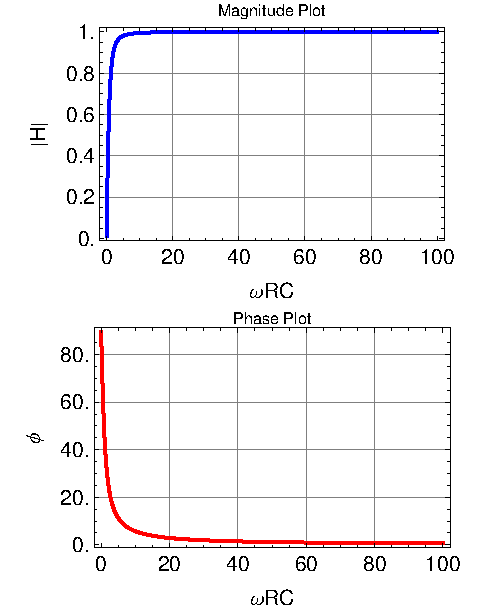
\includegraphics[width=0.7\textwidth]{bodepa_lin.pdf}
  			\caption{Linear Bode plots, $|H|^2=\frac{\omega R C}{1+\omega^2 R^2 C^2},\phi=tan^{-1}(1/\omega RC)$}
  			\label{fig:bodepa_lin}
			\end{figure}
		\end{column}
		\begin{column}{0.5\textwidth}
			\begin{figure}
  			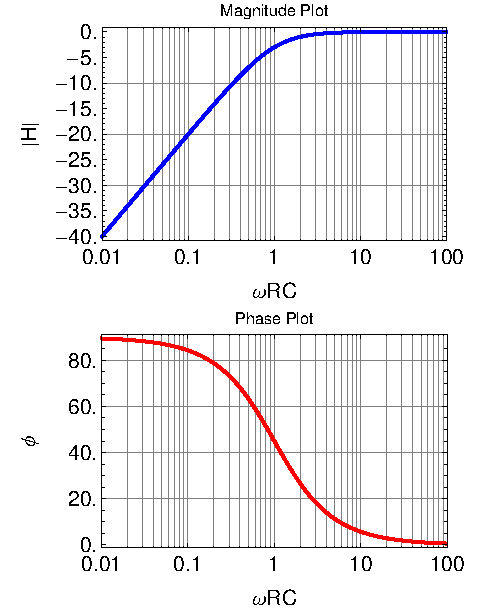
\includegraphics[width=0.7\textwidth]{bodepa_log.pdf}
  			\caption{Log Bode plots, $|H|^2=\frac{\omega R C}{1+\omega^2 R^2 C^2},\phi=tan^{-1}(1/\omega RC)$}
  			\label{fig:bodepa_log}
			\end{figure}
		\end{column}
	\end{columns}
\end{frame}
\subsection{RLC circuit}

\begin{frame}{RLC circuit}
\begin{center}
	\begin{circuitikz}[scale=0.5]
		\node (Xi) at (0.7,0.7) {$V_1$};
		\node (Xf) at (5.7,0.7) {$V_2$};
		\draw [semithick,->] (Xi) -- (0.1,0.1);
		\draw [semithick,->] (Xf) -- (5.1,0.1);
		\draw	to [inductor, o-o, l_=L] ++(2,0)
				to [capacitor, o-o, l_=C] ++(2,0)
				(4,0) to [short,o-o] ++(1,0)
				(4,0) to [resistor, o-o, l=R] ++(0,-2)
				node[ground] {};
	\end{circuitikz}
\end{center}
The KCL equation now reads,
\begin{eqnarray}
v_1(t)=L \frac{di}{dt} + q(t)/C +R i(t)\label{eq:rlc_kcl1}\\
\Rightarrow \frac{1}{L}\frac{dv_1}{dt}=\frac{d^2i}{dt^2} + \textcolor{blue}{\frac{R}{L}} \frac{di}{dt} + \textcolor{blue}{\frac{1}{LC}}i\\
\Rightarrow \frac{1}{L}\frac{dv_1}{dt}=\frac{d^2i}{dt^2} + \textcolor{blue}{\gamma} \frac{di}{dt} + \textcolor{blue}{\omega_0^2} i
\label{eq:rlc_kcl2}
  \end{eqnarray}
Where we defined $\textcolor{blue}{\gamma} \equiv R/L[T^{-1}]$ and $\textcolor{blue}{\omega_0} \equiv 1/LC[T^{-2}]$. Of course we could repeat the process of attempting to find a solution of the form $i(t)=i_0 \cos(\omega t+\phi)$ for a given $v_1(t)=V_1 \cos(\omega t)$. That would work perfectly and you can work out the result. \textbf{We want however a more powerful method for looking at such circuits!}
\end{frame}


\begin{frame}{Complex numbers \& Trigonometric functions}
The connection between complex number and trigonometric functions lies on the so-called Euler's identity,
\begin{equation}
  \exp(ix)=\cos(x)+j\sin(x)
  \label{eq:euler}
\end{equation}
\pause
A simple proof of Euler's identity is given below:
\begin{proof}
Let's define $f(x)=\cos(x)+j\sin(x)$. Therefore $f'(x)=-\sin(x)+j\cos(x)=j[\cos(x)-\frac{1}{j}\sin(x)]$. However $j^2\equiv -1$, $\Rightarrow f'(x)=j[\cos(x)+{j}\sin(x)]=j f(x)\Rightarrow f(x)=\exp(j x)$
\end{proof}
One we are convinced that \ref{eq:euler} is true, we can write the driving term in KCL as $v_1(t)=V_1\cos(\omega t)=\Re(V_1\exp\i\omega t)$. If were to introduce a phase $\phi$ in the driving term, $v_1(t)=V_1\cos(\omega t+\phi)$, the complex exponential representation would follow as $v_1(t)=\Re((\textcolor{red}{V_1\exp j \phi} )\exp j\omega t)$. It is therefore convenient to define a complex amplitude $\tilde{V}_1\equiv\color{red}{V_1\exp j \phi}$ that can incorporate any phase. We use the $\tilde{ }$ to emphasize that $\tilde{V}_1$ is a complex number. The quantity $\tilde{V}_1$ is also known as a \textbf{phasor}; in this case a voltage \textbf{phasor}.
\end{frame}
\begin{frame}
Below we illustrate the geometric relation between a trigonometric waveform in a cartesian plot and its phasor analog in the complex plane. Assuming that the current flowing is $i(t)=\cos(2\pi t)$, we could think of them as the voltage drop in the three basic circuit components:
\begin{eqnarray}
\textcolor{blue}{v_R(t) = R i(t) = R \cos\omega t=\Re (R \exp j\omega t)}\\
\pause
\textcolor{green}{v_C(t) = q(t)/C=\frac{1}{C}\int i(t) dt=\frac{\sin \omega t}{\omega C}=\Re\left(\frac{\exp j \omega t}{j\omega C}\right)}\\
\pause
\textcolor{red}{v_L(t) = L \dt{i}=-L\sin \omega t=\Re (j \omega L \exp j\omega t)}
\end{eqnarray}
\pause
In the figures below we represent these waveforms both in trigonometric  and phasor representations. Note that as time evolves, the phase-relation (angle) between the phasors are constant.
\begin{columns}
	\begin{column}{0.5\textwidth}
		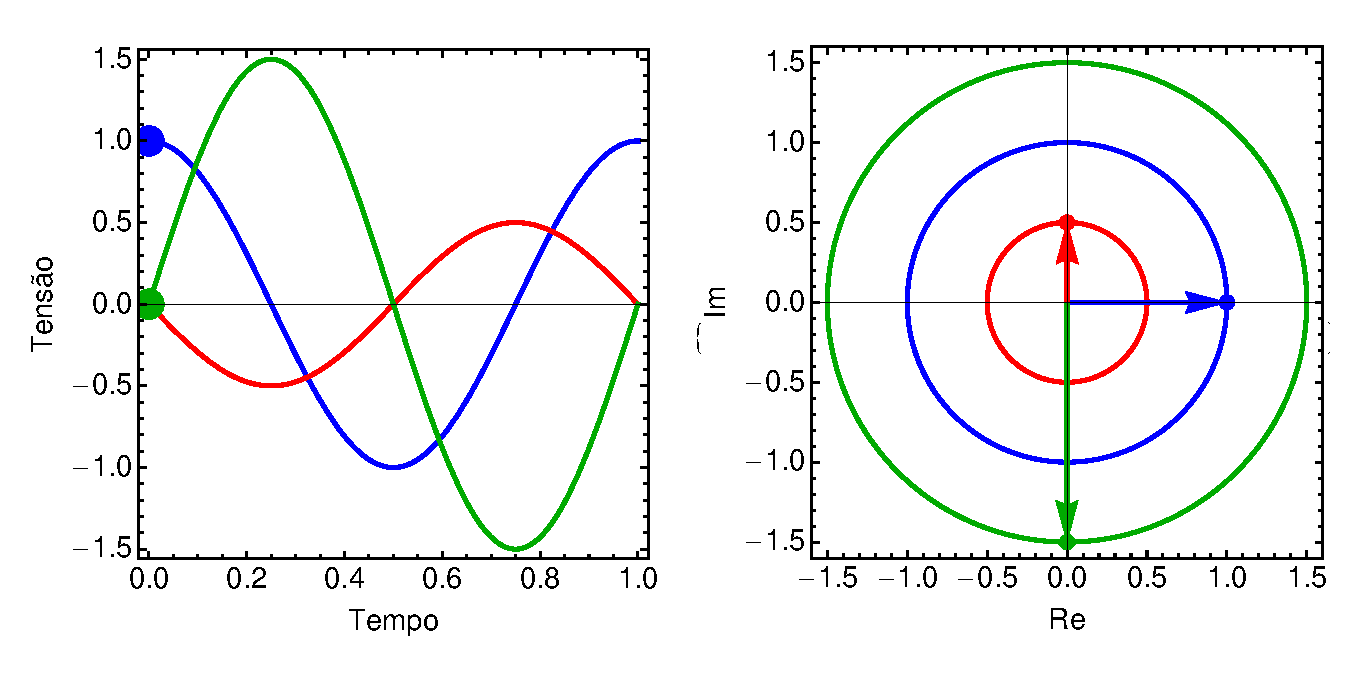
\includegraphics[width=\textwidth]{fasor0.pdf}
	\end{column}
	\begin{column}{0.5\textwidth}
		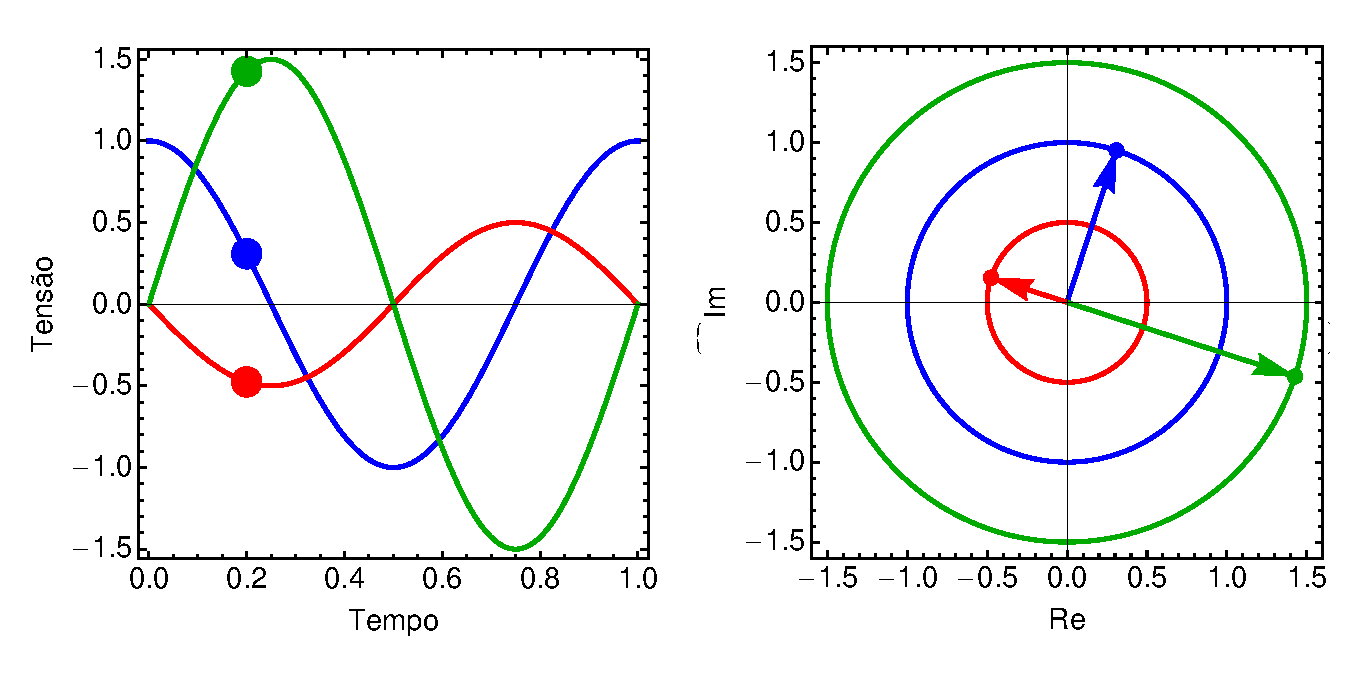
\includegraphics[width=\textwidth]{fasor0p2.pdf}
	\end{column}
\end{columns}
\end{frame}

\begin{frame}
Based on the previous definitions, one would be tempted to write Eq. \ref{eq:rlc_kcl2} in the form,
\begin{equation}
\frac{d^2i}{dt^2} + \gamma \dt{i} + \omega_0^2i=\frac{1}{L}\dt{ }\Re (\tilde{V}_1\ejt)
\label{eq:kcl_rlc_c1}
\end{equation}
Eq. \ref{eq:kcl_rlc_c1} still represents a real physical current, as it should be. Let's assume for a moment however that the RHS (right-hand side) is an actual complex number and drop-off the $\Re()$ operation,
\begin{equation}
\frac{d^2\tilde{i}}{dt^2} + \gamma \dt{\tilde{i}} + \omega_0^2\tilde{i}=\frac{1}{L}\dt{ }(\tilde{V}_1\ejt)
\label{eq:kcl_rlc_c2}
\end{equation}
Since we have a complex RHS, we should expect that the current is also complex; to remember that we wrote $\tilde{i}$ for the current. Now we explore the fact that Eq. \ref{eq:kcl_rlc_c2} is a \textbf{linear ODE} and therefore the superposition principle is valid. From Euler's identity we now we can decompose the RHS into a real and a imaginary component. The same applies for the LHS, $\tilde{i}=\Re(\tilde{i})+j\Im(\tilde{i})$. In order for \ref{eq:kcl_rlc_c2} to be true, both its real and imaginary parts must hold, therefore when we solve Eq. \ref{eq:kcl_rlc_c2} we are actually solving for both the real and imaginary parts of our fictitious imaginary current $\tilde{i}(t)$. The \textbf{actual physical current} can be obtained by taking $i(t)=\Re(\tilde{i}(t))$.
\end{frame}

\begin{frame}
We can now apply the same solution approach we used to solve \ref{eq:rc_1}. After the initial transients the homogeneous equation solution $\tilde{i}_h(t)$ decays and \textbf{the only important contribution is due to} the particular solution $\tilde{i}_p(t)$. Similarly, the ansatz solution is $\tilde{i}_p(t)=\tilde{i}_0 \ejt$. 

Now we will be paid back for all the effort in using the complex exponential. The derivatives of the voltage (RHS)  and current (LHS) are straightforward:
\begin{eqnarray}
\dt{ }(\tilde{V}_1\ejt) = j \omega \textcolor{red}{\tilde{V}_1 \ejt}\\
\dt{\tilde{i}_p}=j \omega \textcolor{red}{\tilde{i}_0 \ejt}\\
\frac{d^2\tilde{i}}{dt^2}=(j \omega)^2 \textcolor{red}{\tilde{i}_0 \ejt}= -\omega^2 \textcolor{red}{\tilde{i}_0 \ejt}
\end{eqnarray}


Substituting these in Eq. \ref{eq:kcl_rlc_c2} we obtain
\begin{equation}
	(-\omega^2 + j\omega \frac{R}{L} +\frac{1}{L^2 C^2})\tilde{i}_0 \ejt = \frac{j \omega}{L}\tilde{V}_1 \ejt
	\label{eq:kcl_rlc_c3}
\end{equation}
In order to Eq. \ref{eq:kcl_rlc_c3} to be valid for all times we must have
\begin{equation}
	\tilde{i}_0=\frac{1}{\textcolor{blue}{R}+j\left(\textcolor{blue}{\omega L-\frac{1}{\omega C}}\right)}\tilde{V}_1
	\label{eq:i0_vs_v1}
\end{equation}

\end{frame}

\begin{frame}
In contrast to the trigonometric function approach, where phase and amplitude equations (\ref{eq:rc_v2final_r}) were obtained separately from the $\cos$ and $\sin$ functions, the complex exponential approach gives us right away both information. 
Eq. \ref{eq:i0_vs_v1} is a complex algebraic relation between current and voltage, resembling Ohm's law ($V=RI$). It is still useful to define a complex analog of resistance, which is known as impedance an denoted by $Z$. Using Eq. \ref{eq:i0_vs_v1} on can write
\begin{equation}
	\boxed{
	\tilde{V}_1=\textcolor{red}{Z(\omega)} \tilde{i}_0
	}
	\label{eq:complex_impedance}
\end{equation}
Where we defined the \textbf{complex impedance} as 
\begin{equation}
\textcolor{red}{Z(\omega)}\equiv \textcolor{blue}{R+jX},
\end{equation}
where $\textcolor{blue}{X=\omega L-\frac{1}{\omega C}}$ is known as reactance of the circuit. The obtain the impedance all we need to do is sum up the individual impedances of the circuit components, in the RLC case 
\begin{equation}
Z=\textcolor{blue}{Z_R}+\textcolor{green}{Z_C}+\textcolor{red}{Z_L}=\textcolor{blue}{R} + (\textcolor{green}{-j(\omega C)})+\textcolor{red}{(j\omega L)},
\end{equation}
\center{It is that easy!}
\end{frame}
\begin{frame}
Another useful quantity is the \textbf{complex admittance}, the reciprocal of the impedance, $Y\equiv Z^{-1}$, therefore,
\begin{equation}
  Y(\omega) = \frac{R}{R^2+X^2}-j\frac{X}{R^2+X^2} = \frac{R}{|Z|}-j\frac{X}{|Z|}
\end{equation}

To illustrate the usefullness of $Z,W$ lets set the AC source as the phase reference (without loss of generality), $\tilde{V}_1=V_1\exp\phi\rightarrow V_1\in\Re$. For example,
\begin{itemize}
\item the physical (\textbf{real}) current amplitude is given by $i_0=|\tilde{i}_0|=|Y||\tilde{V}_1|=\sqrt{R^2+X^2}V_1$
\pause
\item the phase between the AC generator voltage and circuit current is simply $\psi=\tan^{-1}\left(\frac{-X}{R}\right)$
\pause
\item the voltage drop across any element (or combinations) in the circuit with impedance $Z_e$ is given by $\tilde{V}_e=Z_e/Z\tilde{V}_1$
\end{itemize}
 


\end{frame}

%\begin{frame}{Complex numbers \& Trigonometric functions}
%
%  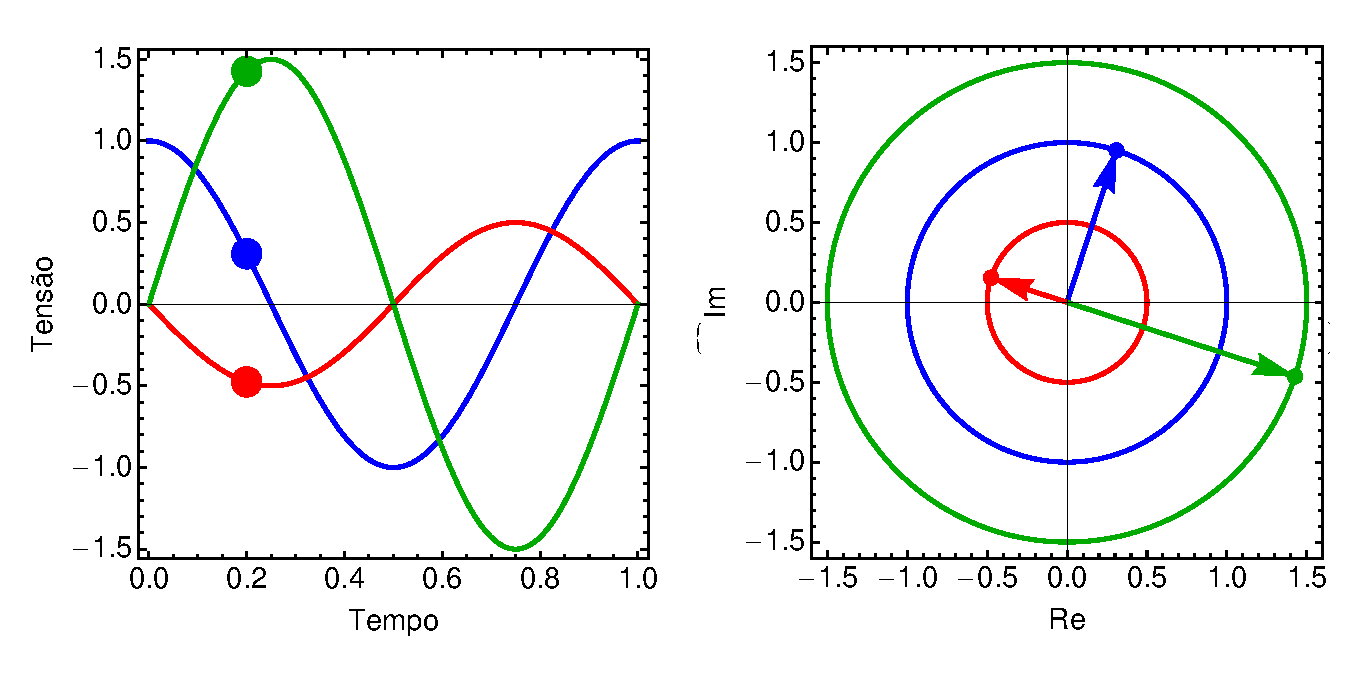
\includegraphics[width=\textwidth,natwidth=100]{fasor0p2.pdf}
%
%\end{frame}

\begin{frame}{Power Dissipation in RLC circuits}
As current and voltage are time-dependent functions, we can define an instantaneous power dissipated in a given circuit component with a voltage drop $v(t)$ as
\begin{equation}
  P(t)=v(t)i(t),
\end{equation}
\pause
where i(t) is the current flowing through the circuit component. \pause Writing $v(t)=v_0\cos(\omega t)$, $i(t)=v_0\cos(\omega t+\phi)$ we obtain,
\begin{equation}
  P(t)=\frac{1}{2}\left(v_0 i_0\cos(\phi)+\cos(2\omega t+\phi)\right),
\end{equation}
\pause
The average power (over one period, $T=2\pi/\omega$) can be obtained as,
\begin{equation}
  \bar{P}\equiv\frac{1}{T}\int_0^{T}P(t)=\frac{1}{2}v_0 i_0\cos(\phi),
\end{equation}
\pause
Two aspects must be noticed from Eq. above
\begin{itemize}
  \item 
\end{itemize}
\end{frame}

\begin{frame}
\begin{columns}
	\begin{column}{0.33\textwidth}		
	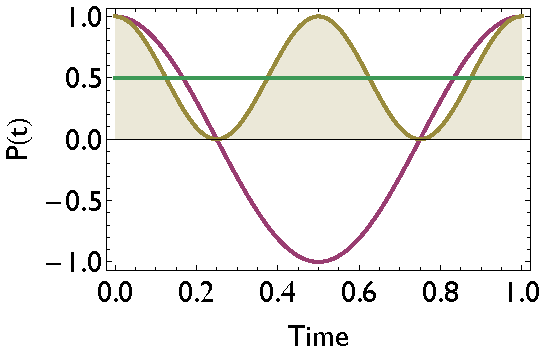
\includegraphics[width=\textwidth]{potencia_instantanea_phi0.pdf}
	\center{	$\phi=0^\circ$}
	\end{column}
	\pause
	\begin{column}{0.33\textwidth}
	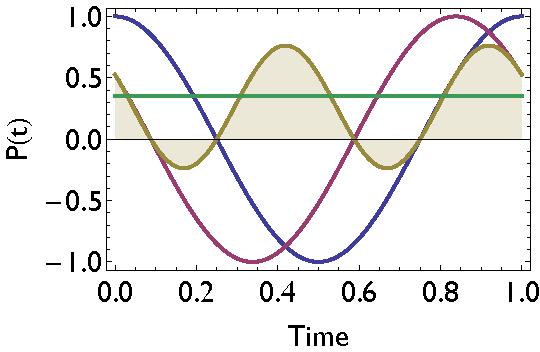
\includegraphics[width=\textwidth]{potencia_instantanea_phi45.pdf}
		\center{	$\phi=0^\circ$}
	\end{column}
	\pause
	\begin{column}{0.33\textwidth}
	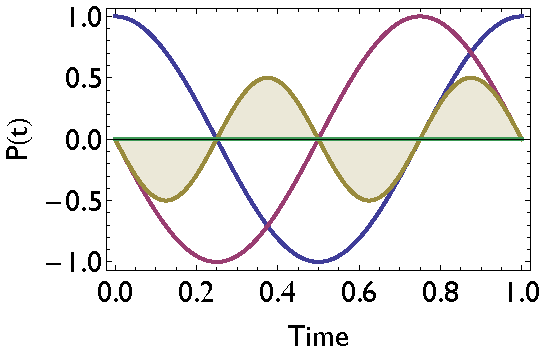
\includegraphics[width=\textwidth]{potencia_instantanea_phi90.pdf}
		\center{	$\phi=90^\circ$}
	\end{column}
\end{columns}

\pause
	\begin{columns}
		\begin{column}{0.5\textwidth}
		In figure we show the time dependence of the instantaneous power (yellow curve) together with a unit voltage 	($v_0=1$, blue curve) and a unit current ($i_0=1$, red curve) and $\phi=45^{\circ}$. The green curve shows the 	average power $\bar{P}$. 
		\end{column}
		\begin{column}{0.5\textwidth}
			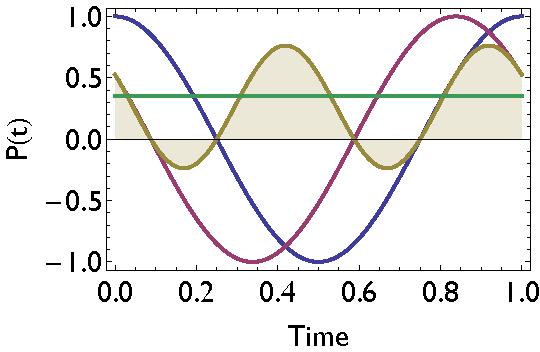
\includegraphics[width=.8\textwidth]{potencia_instantanea_phi45.pdf}
		\end{column}
	\end{columns}
From Ohm's law we now that current can be easily measured from the voltage drop across the circuit's resistor $i(t)=\frac{1}{R}v_R(t)$
\end{frame}

\begin{frame}
	\begin{columns}
		\begin{column}{0.5\textwidth}
			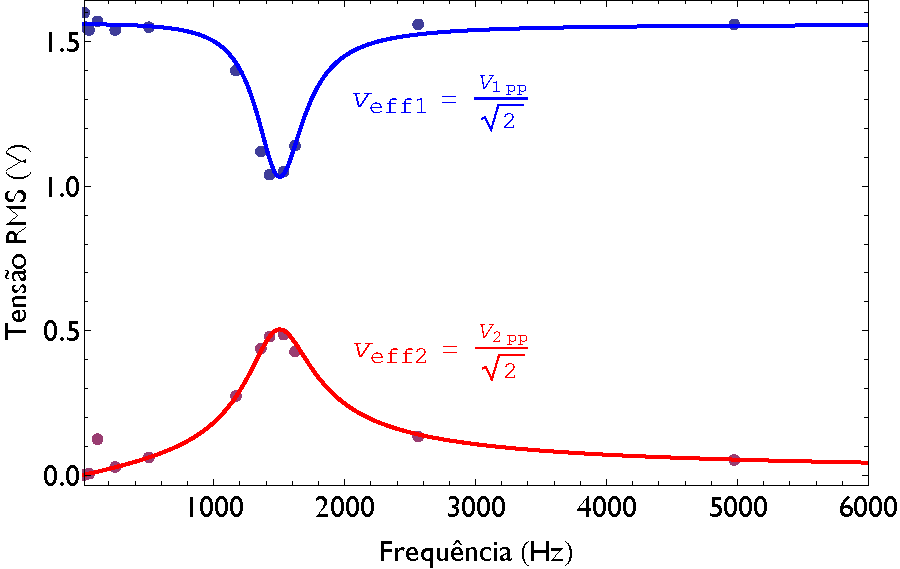
\includegraphics[width=\textwidth]{v1_v2_eff_rlc.pdf}
		\end{column}
		\begin{column}{0.5\textwidth}
			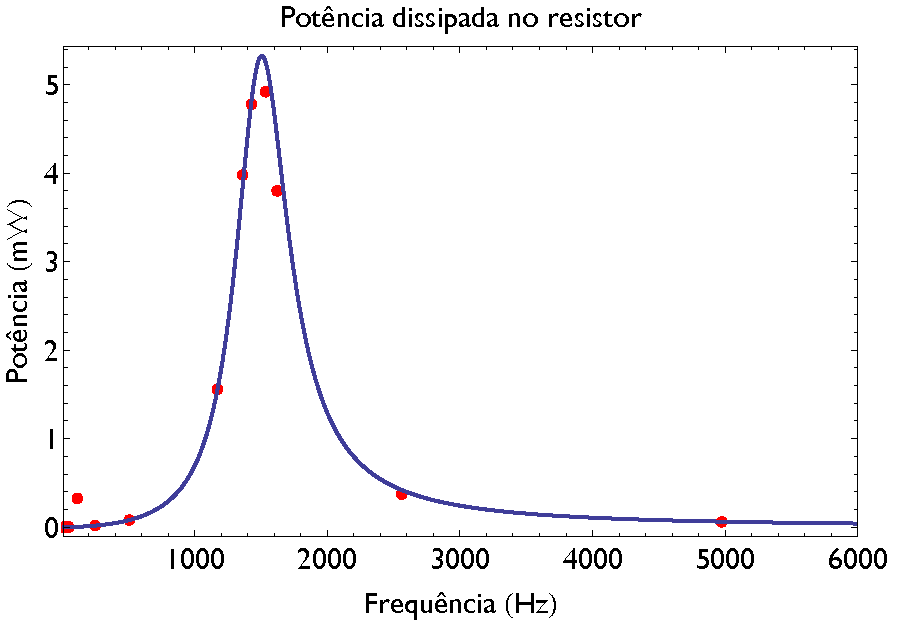
\includegraphics[width=\textwidth]{pdiss_rlc.pdf}
		\end{column}
	\end{columns}
\pause
    E=mc\\
    \pause
    E=mc2\\
    \pause
    E=mc3\\
\end{frame}



\begin{frame}
\label{fr:appendix1}
Test\hyperlink{twoport}{\beamerbutton{here}}.
\end{frame}

%Bilbiography
\begin{frame}{Bibliography}
	\bibliographystyle{plain}
	\bibliography{references}
\end{frame}



\end{document}

